\documentclass[conference]{IEEEtran}
\IEEEoverridecommandlockouts
% The preceding line is only needed to identify funding in the first footnote. If that is unneeded, please comment it out.
\usepackage{cite}
\usepackage{amsmath,amssymb,amsfonts}
\usepackage{algorithmic}
\usepackage{graphicx}
\usepackage{textcomp}
\usepackage{xcolor}

\usepackage{tabularx}

\def\BibTeX{{\rm B\kern-.05em{\sc i\kern-.025em b}\kern-.08em
    T\kern-.1667em\lower.7ex\hbox{E}\kern-.125emX}}
\begin{document}

\title{An Overview on Wireless Body Area Networks}

\author{\IEEEauthorblockN{Rudy Berton, Vassilik\'\i \ Menarin }
	
\IEEEauthorblockA{Department of Mathematics ``Tullio Levi-Civita'' \\ University of Padua \\ Padua, Italy \\ \textit{rudy.berton@studenti.unipd.it, vassiliki.menarin@studenti.unipd.it }}
}

\maketitle

\begin{abstract}
Wireless Body Area Networks (WBAN) is a recent wireless technology that presents its main application in medical field with the use of sensors that work in close vicinity to, on or inside a human body. Through the years, two main standards have been established by a task group to define this technology: IEEE 802.15.4 and IEEE 802.15.6. The purpose of this paper is to give a general overview of the technology employed in WBANs, describing the standards with their differences between Physical and Mac layers, to talk about the different fields in which WBANs can be applied and the issues and challenges that may arise when working with these networks.
\end{abstract}
\hfill
%
%\begin{IEEEkeywords}
%Da mettere??? %component, formatting, style, styling, insert
%\end{IEEEkeywords}

\section{Introduction}
The interest in developing wireless networks built around humans, mainly for an easy and quick way to help monitor health and physiology, has significantly grown in recent years: there is now a higher demand for these kind of communications, that have recently become possible thanks to technological advances.

In particular, the minimization of components and the creation of very-low-power wireless technologies have opened new possibilities for the development of small, personal wireless networks. Furthermore, non-invasive technologies as well as technologies compatible with human physiology are very sought after.

Wireless Body Area Networks (WBANs) have been developed as a new wireless technology with promising applications in many fields, mainly healthcare, but also athletic training, secure authentication and safety.

A WBAN is a network that connects tiny nodes, usually sensors and/or actuators to the human body. The wireless sensors are usually placed in, on or around a person’s body. From there, they connect to router nodes that receive and elaborate the data transmitted. Since these router nodes are intended to be placed around the wearer, the sensor nodes don’t need to cover wide ranges, averaging around 2m. From there, the data may ultimately be sent to centralized centers and databases. Figure \ref{fig_WBAN_arch} shows the general architecture of a WBAN.

\begin{figure}[htbp]
\centering
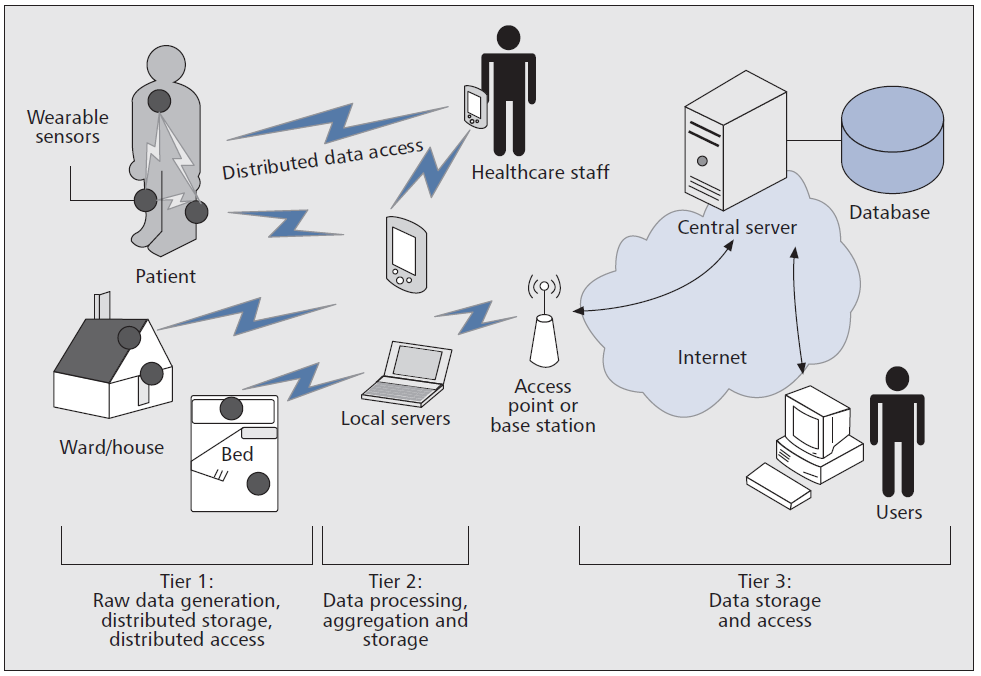
\includegraphics[width=0.9\linewidth]{img/WBAN_arch.png}
\caption{The general architecture of WBANs}
\label{fig_WBAN_arch}
\end{figure}

Since they are based on sensors that gather and elaborate data, WBANs may be considered similar to sensor networks but, due to their unique characteristics, they pose some new technical challenges \cite{cao2009enabling}. Some of the main differences between WBANs and conventional sensor networks are listed in Table \ref{tab1}.

\begin{table}[htbp]
	\caption{Main differences between WSNs and WBANs}
	%\begin{center}
	\begin{tabularx}{0.5\textwidth}{r|X|X|}
	% \begin{tabular}{r|c|c|}
	 & \textbf{WSN} & \textbf{WBAN} \\
	\hline
	Architecture & Every node is both a sensor and a router & Two categories of nodes: sensor/actuators placed in or on the human body and router nodes around them \\
	\hline
	Density & May present high redundancy for a better fault tolerance & Usually low \\
	\hline
	Data rate & Usually used for monitoring irregular events & Human physiological activities may vary in a periodic manner, this may lead to stable data rates \\
	\hline
	Latency	& It may be necessary to maximize battery life in a WSN at the expense of higher latency & Reduce latency even if it impacts battery savings (replacements of batteries may be easy) \\
	\hline
	Mobility & Stationary nodes & Wearers move around \\
	\hline
	\end{tabularx}
	\label{tab1}
	%\end{center}
	\end{table}

We will now discuss some of WBANs' most promising applications. Then we will discuss the different standards that have already been set for this kind of networks and their main differences. Finally, we’ll give an overview of the challenges these network pose.


\section{WBAN Applications and Devices}
The employment of Wireless Body Area Networks was initially mainly focused on the medical field, nevertheless in the last years, starting from these initial discoveries, they have been used to introduce some innovations in non-medical fields too.

Still, the most common application of this technology remains healthcare, where WBAN is used to collect biomedical signals monitoring patients with health problems remotely and continually. 
Knowing the patient's history and coupling this knowledge with this type of applications can reduce medical accidents and increase public safety alerting medical personnel in time. Some parameters monitored are heartbeat, body temperature and blood pressure. This is possible thanks to wearable applications (e.g. ECG) while implanted applications are used to monitor more particular diseases (e.g. diabetes, cancer) and can be implanted directly under the skin or in the bloodstream.

Some non-medical fields in which WBAN is recently being employed are the sports, entertainment and military environment. Both in the first and last case this technology can improve performances of athletes and soldiers keeping a log of physiological data, as well as detect life threatening situations in military context. In the entertainment environment WBANs can be used for different purposes, for example to register body motions of actors during the making of a film.

There are three classes of devices that constitute WBANs and allow its applications: wireless sensor nodes, actuators and wireless personal devices. The first type concerns components, wearable or implantable, that provide wireless monitoring of people or environment, communicating physiological parameters to other devices. Indeed, the work of actuators depends on the data received: if sensors detect an abnormal parameter, actuator administer medicine to the patient. Finally, a Personal Device (PD) is the device responsible for the communication between sensors, actuators and cellular phone through wireless connection \cite{salayma2017wireless}.


\section{WBAN Standards}
Two are the most known standards created as solution for Wireless Body Area Networks. The first one is IEEE 802.15.4, developed in 2003 and mainly thought for low-rate and low-power Wireless Personal Area Networks (WPAN), later adapted to operate around the human body with a WBAN. The second one is IEEE 802.15.6 and it was born in 2007 abd developed to be a good solution for the WBAN right from the beginning. Its final version was published in 2012 and nowadays is the most widely used standard in WBAN technologies.

These solutions have a different structure in Physical layer (PHY) and Medium Access Control layer (MAC) as we will see below.


\subsection{IEEE 802.15.4}
The topology thought for the IEEE 802.15.4 standard considers devices that consume minimal power in a WPAN and can cover an area of 10 meters using unlicensed radio bands (ISM). Each device represents a node in the network and can have two possible roles during the communications: a coordinator node, with specific tasks to fulfill, or a simple node that only sends/receives information.

The PHY layer presents 27 channels divided in three different frequency bands and interacts with the MAC layer after the selection of the right channel. Moreover, the PHY level controls the activation/deactivation of radio transceivers, the quality of the links, the transmission and reception of packets over the medium and the estimation of the inbound signal power.

The standard's structure allows MAC layer to operate in two different modes, beacon-enabled or beacon-less, using three different access schemes in the exchange of packets: unslotted carrier sensing multiple access with collision avoidance (CSMA-CA), a slotted version of the same one and the contention free period scheme (CFP).
\newline

\textit{Beacon-enabled mode:} There is a coordinator node that periodically transmits a beacon, defining a superframe that starts with a beacon and ends with the next one. Each beacon contains information about the identification and the synchronization of the PAN in addition to the structure of the superframe. The remaining part is called Contention Access Period (CAP) and is used for data transmission made by nodes through the channel using the slotted CSMA/CA for a correct synchronization. Moreover, the coordinator could reserve up to seven slots after CAP in the superframe, called Guaranteed Time Slots (GTS). These slots can be assigned to devices that have to run their applications without the contention with other devices. The GTS form the CFP that works in Time Division Multiple Access (TDMA) [fig. \ref{fig_beaconenabled}].
\newline

\begin{figure}[htbp]
	\centering
	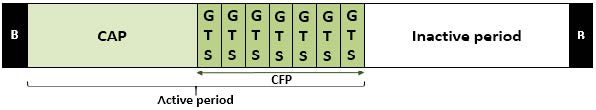
\includegraphics[width=0.9\linewidth]{img/beaconSuperframe.jpg}
	\caption{Superframe in Beacon-enabled mode of standard IEEE~802.15.4}
	\label{fig_beaconenabled}
\end{figure}\



\textit{Beacon-less mode:} No superframe is defined because there isn't any transmission of beacons for the synchronization; only random access is available and for this reason the transmission can not be guarantee and no GTS slot can be reserved. It implies the use of an unslotted version of CSMA-CA before the transmission of data. Devices that want to send data have to pick a random backoff delay and, when it expires, they have to perform a clear channel assessment (CCA): listen if the channel is idle and transmit or pick a new backoff delay to try again in the next transaction. 
\newline

Both the slottend and unslotted CSMA-CA algorithms are only used for data transaction and not for beacon frames, acknowledgment or CFP transmissions and definition of the maximum number of backoffs that can fail before the channel is declared inaccessible. Indeed, in beacon-enabled mode, when the device performs a CCA, after the random backoff delay, if the channel is idle the device decides to repeat the CCA for a number of backoff units in accordance to the value of the contention window (CW) before it transmits. During all the backoff units of CW, if channel is idle, the device can transmit the data, otherwise it has to restart with a new backoff delay. 

In this type of networks two types of data transactions are possible: from coordinator to devices or vice versa. In the former, when the coordinator informs the target device of the data through beacon, the receiver replies that it is ready by sending a request back to the coordinator (using slotted CSMA-CA). The coordinator can now select a free slot to start the transmission. In the latter case, when the coordinator receives data from the device, in a similar way as explained above, it could confirm the successful reception by sending back an acknowledgment \cite{li2009performance}.


\subsection{IEEE 802.15.6}
Several years after IEEE 802.15.4,the definition of a new standardization of WBAN to optimize the low-power nodes that handle the applications started.

The new 802.15.6 standard defines a MAC layer that supports not one but three operational PHYs layers, each one with an hub (or coordinator) and a total number of at most 64 nodes that are organized into one-or-two-hop star topology. A brief description of the physical layers follows:
\newline

\textit{Narrowband PHY}. It is responsible for the activation/deactivation of the radio transceiver, clear channel assessment and data reception/transmission; it defines the Physical Protocol Data Unit (PPDU) frame that includes three components: 
\begin{itemize}
	\item[-] Physical Layer Convergence Procedure (PLCP) preamble is composed of two sequences: the first one is used for coarse time synchronization, carrier-offset recovery and packet detection, the second instead is used for fine time synchronization.
	\item[-] PLCP header contains a PHY header, with several fields used to convey information to the receiver for a successful decoding and some parity check bits used for error detection and error correction of PHY header.
	\item[-] Physical-layer Service Data Unit (PSDU), transmitted for last, contains a MAC header, a MAC frame body and a Frame Check Sequence (FCS).
\end{itemize}
\hfill

\textit{Ultra Wideband PHY}. It supports 11 channels in low and high band with different frequencies and has two modes of operation: default mode and high Quality of Service mode, thought for high priority medical applications. The aim of UWB is to achieve high performance, low complexity and low power consumption. The PPDU frame for this PHY layer consists of the Synchronization Header (SHR) with the same task of PLCP plus the start-of-frame delimiter (SFD) used for frame synchronization; a PHY Header (PHR) that conveys information (about the data rate of the PSDU and length of payload) used by the receiver to decode the PSDU and a third part that defines the frame, similar to the Narrowband one. However, the disposition of parity check bits for error correction of MAC frame body changes.
\newline

\textit{Human Body Communications PHY}. Similar to NB PHY, the packet contains a PLCP preamble, SFD, PLCP header with control and error detection/correction bits and at last PSDU. In this PHY, the preamble sequence is transmitted four times to ensure packet synchronization, while SFD is transmitted once.
\newline

For the MAC layer, the standard defines a channel division into beacon periods (also called superframes) of equal length made by hubs. They transmit a beacon to define the superframe boundaries and allocate the slots that are used for data transmission. Generally a hub transmits a beacon in each active superframe and when beacons are not used the boundaries of superframe are defined by a polling action.

The frame in the MAC layer is formed by a header, a frame body with maximum length of 255 bytes and the Frame Check Sequence at last. The MAC Header includes a control field that controls information about the frame, the sender and recipient identification and the WBAN ID field with information about the network. In addition to the payload, in the MAC frame body there are bits with the aim of assessing the freshness, authenticity and integrity of the message.

IEEE 802.15.6 supports three different communication modes: \textit{Beacon Mode with Superframe Boundaries, Nonbeacon Mode with and without Superframe Boundaries}. In the first mode (fig. \ref{fig_beaconModeSuperframe}), mostly used in medical applications, the superframe structure is divided into Exclusive Access Phases (EAPs), used to transfer high-priority or emergency traffic, Random Access Phases (RAPs), a Contention Access Phase (CAP), both used for regular traffic and Managed Access Phases (MAPs or TypeI/II phases) provided for reservation of transmission periods or for unplanned traffic. When superframe boundaries are defined in non beacon mode the hub operates during the MAP periods only, in the other case instead the hub provides only unscheduled Type II polled allocation because each node establishes its own time base independently.

\begin{figure}[htbp]
	\centering
	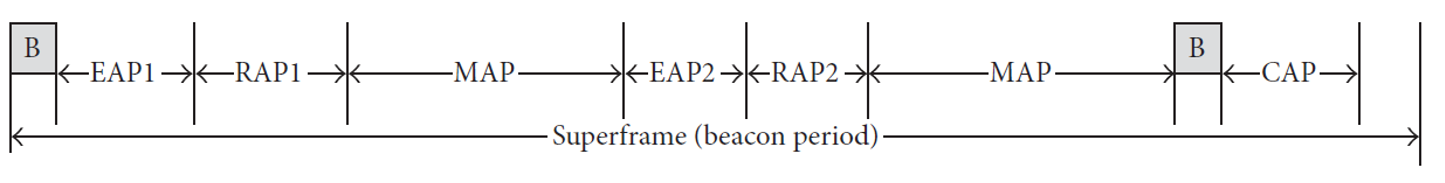
\includegraphics[width=0.9\linewidth]{img/beaconModeSuperframe.png}
	\caption{Beacon mode with superframes of standard IEEE~802.15.6}
	\label{fig_beaconModeSuperframe}
\end{figure}

The access mechanism used in each period of the superframe presents three categories. The \textit{Random Access Mechanism}, used in EAP, RAP and CAP periods, define the use of slotted Aloha or CSMA/CA protocol by the coordinator for the resource allocation. \textit{Improvised and Unscheduled Access Mechanism} is used when hub needs an improvised access to send poll or post commands without a notice in beacon or nonbeacon modes, outside the scheduled allocation interval. \textit{Scheduled and Scheduled-Polling Access Mechanism} instead is used to schedule the allocation of slots in one or multiple upcoming superframes (also called 1-periodic or m-periodic allocations). \cite{kwak2010overview} \cite{ullah2013review}

\subsection{Comparison between WBAN standards}
Table \ref{tab2} \cite{salayma2017wireless} summarizes the main differences in the designs of standards IEEE 802.15.4 and IEEE 802.15.6.

\begin{table}[htbp]
	\caption{A comparison between IEEE 802.15.4 and IEEE 802.15.6}
	%\begin{center}
	\begin{tabularx}{0.5\textwidth}{X|X|X|}
		% \begin{tabular}{r|c|c|}
		\textbf{Criteria} & \textbf{IEEE 802.15.4} & \textbf{IEEE 802.15.6} \\
		\hline
		Network type & WPAN &  WBAN: NB, UWB and HBC\\
		\hline
		MAC modes &  Beacon/Non beacon mode with/without superframe & Superframe with/without beacon mode \\
		\hline
		Access mechanism &  Random access (with contention), scheduled access (without contention) & Contention based random access or connection oriented contention-free \\
		\hline
		Contention access resource allocation procedure	& Slotted and unslotted CSMA/CA & CSMA/CA slotted Aloha \\
		\hline
		Specific Access for prioritised traffic & No & Yes (EAP) \\
		\hline
	\end{tabularx}
	\label{tab2}
	%\end{center}
\end{table}

There have been some tests and evaluations on the two standards described to better understand how to employ them in WBANs and which one is better fitted for real-life scenarios. Even though IEEE 802.15.6 was specifically designed for WBANS, tests done in a simulation environments (Castalia for both \cite{nabila2019qos} and \cite{toumanari2014performance}) show how 802.15.4 outperforms 802.15.6 in terms of throughput and energy consumption. Indeed, the number of received packets in IEEE 802.15.4 is greater since it uses TDMA technology that mitigates the number of packet collision; in EAP and RAP periods instead, for standard 802.15.6, the use of CSMA/CA access procedure for resource allocation leads to a higher collision probability for nodes with same priority. More specifically, 802.15.4 seems overall more suited for communications in low traffic rates conditions. On the other hand, 802.16.6 shows better performances when it comes to packet delivery latency and seems to work better in high traffic rate scenarios.

One proposal \cite{nabila2019qos} is to use IEEE 802.15.4 for non-time critical sensor requiring low data rates while favoring IEEE 802.15.6 for sensors with high data rates and in time critical applications. 

\section{Challenges and open research issues}
To design efficient and usable WBANs, we have to overcome some important challenges. Since WBANs may be used in different applications, the issues we are facing may also vary a lot. Here we analyze the general challenges and research issues one has to consider when designing a WBAN \cite{cao2009enabling}, even though they may not all be pertinent at the same time.

\subsection {Physical characteristics of nodes}
Since the nodes are going to be implemented on, if not inside, human bodies, it is crucial to consider how they are built. One needs to carefully evaluate their size, material and compatibility with the human body. Furthermore, many people may find the implant of a sensor inside their body invasive, and refuse it. Thus, sensor placed on the skin may be preferable. Finally, one needs to answer concerns regarding the electronic and magnetic energy absorbed by human tissues.

\subsection {WBAN specific issues}
Overall, WBANs would benefit for more research and improved models to help predict their unique behavior in realistic environments. For example, how is the signal propagation being affected by the physical characteristics of the human body? Are there going to be issues when considering a moving wearer? Also, power management, sensor calibration, management of resources may be handled in new, different ways from the ones already in use in other kind of networks.

\subsection {Power Supply}
While batteries may be easy to replace in devices situated outside the human bodies, remote battery recharging becomes not-negotiable for devises implemented directly inside the human body.

\subsection {Device Interoperability}
Different devices, from different manufacturers and monitoring different phenomena may be implemented at the same time on a single wearer. All these devices need to be able to operate without interfering with each other. In same cases, they may need to exchange data between them. The setting of some common standards may greatly help with device compatibility. 

\subsection {Privacy and Security issues}
Security may be the greatest challenge for WBAN and it’s strongly required due to the nature of the data exchanged, especially in medical applications. Since WBANs deal with very personal information, there is a strong need to ensure data privacy and a reliable authentication in the whole data transfer process. 

Not only this, data also needs to be confidential, uncorrupted and dependable. Finding the right balance is a very delicate matter and security may conflict with many other aspects. Depending on the system we are building we may need to sacrifice efficiency or usability for an increased security. 

Paper \cite{li2010data} gives an overview on all the different security issues involved when dealing with WLANs in healthcare, here we list some of the most common practical issues concerning security:
	\begin{itemize}
		\item[-] Security and Efficiency: the devices involved in WBANs are very small and may lack the storage capabilities and power supplies needed for strong cryptographic computations required to ensure security. Efficiency may be sacrificed dedicating more power to the security operations
		\item[-]  Security and Safety: the devices may carry vital information on the wearer’s health which may become inaccessible in time of need if the wearer is unconscious or unresponsive. There needs to be a way to ensure strong security as well as privacy while, at the same time, allowing flexible access to qualified, legitimate, medical staff. There has been some research in this regard (\cite{li2010data}) but it's still a challenging requirement
		\item[-] Security and Usability: the main aim of medical WBANs is to simplify health monitoring. That means that even non-qualified people should be able to manage their own devices, at least at a basic level. When configuration and setup of the devices becomes too technical, people may feel discouraged and prefer other solutions. On the other hand, if we try to increase usability by omitting some manual configuration steps, this may lead to looser security policies.
	\end{itemize}


\section{Conclusions}
WBAN is an emerging and promising technology that may bring huge changes in people’s lives. In order to improve this technology a coordinated effort between different fields may be required: proposals may come not only from computer science, but also from biology and the design of new materials. 

We gave an overview of WBANs' many applications and the steps that have already been taken to try and standardize this technology. While WBANs may be used in many different fields, arguably, their most interesting use is healthcare, through what is often termed e-healthcare. E-Healthcare is also the field that poses the biggest challenges, mainly in data security and privacy.

In conclusion, WBAN technology, while still requiring thorough research and studies before it can be widely applied, may lead to very important developments in our everyday lives. 

%\section{Ease of Use}
%
%\subsection{Maintaining the Integrity of the Specifications}
%
%The IEEEtran class file is used to format your paper and style the text. All margins, 
%column widths, line spaces, and text fonts are prescribed; please do not 
%alter them. You may note peculiarities. For example, the head margin
%measures proportionately more than is customary. This measurement 
%and others are deliberate, using specifications that anticipate your paper 
%as one part of the entire proceedings, and not as an independent document. 
%Please do not revise any of the current designations.
%
%\section{Prepare Your Paper Before Styling}
%Before you begin to format your paper, first write and save the content as a 
%separate text file. Complete all content and organizational editing before 
%formatting. Please note sections \ref{AA}--\ref{SCM} below for more information on 
%proofreading, spelling and grammar.
%
%Keep your text and graphic files separate until after the text has been 
%formatted and styled. Do not number text heads---{\LaTeX} will do that 
%for you.
%
%\subsection{Abbreviations and Acronyms}\label{AA}
%Define abbreviations and acronyms the first time they are used in the text, 
%even after they have been defined in the abstract. Abbreviations such as 
%IEEE, SI, MKS, CGS, ac, dc, and rms do not have to be defined. Do not use 
%abbreviations in the title or heads unless they are unavoidable.
%
%\subsection{Units}
%\begin{itemize}
%\item Use either SI (MKS) or CGS as primary units. (SI units are encouraged.) English units may be used as secondary units (in parentheses). An exception would be the use of English units as identifiers in trade, such as ``3.5-inch disk drive''.
%\item Avoid combining SI and CGS units, such as current in amperes and magnetic field in oersteds. This often leads to confusion because equations do not balance dimensionally. If you must use mixed units, clearly state the units for each quantity that you use in an equation.
%\item Do not mix complete spellings and abbreviations of units: ``Wb/m\textsuperscript{2}'' or ``webers per square meter'', not ``webers/m\textsuperscript{2}''. Spell out units when they appear in text: ``. . . a few henries'', not ``. . . a few H''.
%\item Use a zero before decimal points: ``0.25'', not ``.25''. Use ``cm\textsuperscript{3}'', not ``cc''.)
%\end{itemize}
%
%\subsection{Equations}
%Number equations consecutively. To make your 
%equations more compact, you may use the solidus (~/~), the exp function, or 
%appropriate exponents. Italicize Roman symbols for quantities and variables, 
%but not Greek symbols. Use a long dash rather than a hyphen for a minus 
%sign. Punctuate equations with commas or periods when they are part of a 
%sentence, as in:
%\begin{equation}
%a+b=\gamma\label{eq}
%\end{equation}
%
%Be sure that the 
%symbols in your equation have been defined before or immediately following 
%the equation. Use ``\eqref{eq}'', not ``Eq.~\eqref{eq}'' or ``equation \eqref{eq}'', except at 
%the beginning of a sentence: ``Equation \eqref{eq} is . . .''
%
%\subsection{\LaTeX-Specific Advice}
%
%Please use ``soft'' (e.g., \verb|\eqref{Eq}|) cross references instead
%of ``hard'' references (e.g., \verb|(1)|). That will make it possible
%to combine sections, add equations, or change the order of figures or
%citations without having to go through the file line by line.
%
%Please don't use the \verb|{eqnarray}| equation environment. Use
%\verb|{align}| or \verb|{IEEEeqnarray}| instead. The \verb|{eqnarray}|
%environment leaves unsightly spaces around relation symbols.
%
%Please note that the \verb|{subequations}| environment in {\LaTeX}
%will increment the main equation counter even when there are no
%equation numbers displayed. If you forget that, you might write an
%article in which the equation numbers skip from (17) to (20), causing
%the copy editors to wonder if you've discovered a new method of
%counting.
%
%{\BibTeX} does not work by magic. It doesn't get the bibliographic
%data from thin air but from .bib files. If you use {\BibTeX} to produce a
%bibliography you must send the .bib files. 
%
%{\LaTeX} can't read your mind. If you assign the same label to a
%subsubsection and a table, you might find that Table I has been cross
%referenced as Table IV-B3. 
%
%{\LaTeX} does not have precognitive abilities. If you put a
%\verb|\label| command before the command that updates the counter it's
%supposed to be using, the label will pick up the last counter to be
%cross referenced instead. In particular, a \verb|\label| command
%should not go before the caption of a figure or a table.
%
%Do not use \verb|\nonumber| inside the \verb|{array}| environment. It
%will not stop equation numbers inside \verb|{array}| (there won't be
%any anyway) and it might stop a wanted equation number in the
%surrounding equation.
%
%\subsection{Some Common Mistakes}\label{SCM}
%\begin{itemize}
%\item The word ``data'' is plural, not singular.
%\item The subscript for the permeability of vacuum $\mu_{0}$, and other common scientific constants, is zero with subscript formatting, not a lowercase letter ``o''.
%\item In American English, commas, semicolons, periods, question and exclamation marks are located within quotation marks only when a complete thought or name is cited, such as a title or full quotation. When quotation marks are used, instead of a bold or italic typeface, to highlight a word or phrase, punctuation should appear outside of the quotation marks. A parenthetical phrase or statement at the end of a sentence is punctuated outside of the closing parenthesis (like this). (A parenthetical sentence is punctuated within the parentheses.)
%\item A graph within a graph is an ``inset'', not an ``insert''. The word alternatively is preferred to the word ``alternately'' (unless you really mean something that alternates).
%\item Do not use the word ``essentially'' to mean ``approximately'' or ``effectively''.
%\item In your paper title, if the words ``that uses'' can accurately replace the word ``using'', capitalize the ``u''; if not, keep using lower-cased.
%\item Be aware of the different meanings of the homophones ``affect'' and ``effect'', ``complement'' and ``compliment'', ``discreet'' and ``discrete'', ``principal'' and ``principle''.
%\item Do not confuse ``imply'' and ``infer''.
%\item The prefix ``non'' is not a word; it should be joined to the word it modifies, usually without a hyphen.
%\item There is no period after the ``et'' in the Latin abbreviation ``et al.''.
%\item The abbreviation ``i.e.'' means ``that is'', and the abbreviation ``e.g.'' means ``for example''.
%\end{itemize}
%An excellent style manual for science writers is \cite{b7}.
%
%\subsection{Authors and Affiliations}
%\textbf{The class file is designed for, but not limited to, six authors.} A 
%minimum of one author is required for all conference articles. Author names 
%should be listed starting from left to right and then moving down to the 
%next line. This is the author sequence that will be used in future citations 
%and by indexing services. Names should not be listed in columns nor group by 
%affiliation. Please keep your affiliations as succinct as possible (for 
%example, do not differentiate among departments of the same organization).
%
%\subsection{Identify the Headings}
%Headings, or heads, are organizational devices that guide the reader through 
%your paper. There are two types: component heads and text heads.
%
%Component heads identify the different components of your paper and are not 
%topically subordinate to each other. Examples include Acknowledgments and 
%References and, for these, the correct style to use is ``Heading 5''. Use 
%``figure caption'' for your Figure captions, and ``table head'' for your 
%table title. Run-in heads, such as ``Abstract'', will require you to apply a 
%style (in this case, italic) in addition to the style provided by the drop 
%down menu to differentiate the head from the text.
%
%Text heads organize the topics on a relational, hierarchical basis. For 
%example, the paper title is the primary text head because all subsequent 
%material relates and elaborates on this one topic. If there are two or more 
%sub-topics, the next level head (uppercase Roman numerals) should be used 
%and, conversely, if there are not at least two sub-topics, then no subheads 
%should be introduced.
%
%\subsection{Figures and Tables}
%\paragraph{Positioning Figures and Tables} Place figures and tables at the top and 
%bottom of columns. Avoid placing them in the middle of columns. Large 
%figures and tables may span across both columns. Figure captions should be 
%below the figures; table heads should appear above the tables. Insert 
%figures and tables after they are cited in the text. Use the abbreviation 
%``Fig.~\ref{fig}'', even at the beginning of a sentence.
%
%\begin{table}[htbp]
%\caption{Table Type Styles}
%\begin{center}
%\begin{tabular}{|c|c|c|c|}
%\hline
%\textbf{Table}&\multicolumn{3}{|c|}{\textbf{Table Column Head}} \\
%\cline{2-4} 
%\textbf{Head} & \textbf{\textit{Table column subhead}}& \textbf{\textit{Subhead}}& \textbf{\textit{Subhead}} \\
%\hline
%copy& More table copy$^{\mathrm{a}}$& &  \\
%\hline
%\multicolumn{4}{l}{$^{\mathrm{a}}$Sample of a Table footnote.}
%\end{tabular}
%\label{tab1}
%\end{center}
%\end{table}
%
%\begin{figure}[htbp]
%\centerline{\includegraphics{fig1.png}}
%\caption{Example of a figure caption.}
%\label{fig}
%\end{figure}
%
%Figure Labels: Use 8 point Times New Roman for Figure labels. Use words 
%rather than symbols or abbreviations when writing Figure axis labels to 
%avoid confusing the reader. As an example, write the quantity 
%``Magnetization'', or ``Magnetization, M'', not just ``M''. If including 
%units in the label, present them within parentheses. Do not label axes only 
%with units. In the example, write ``Magnetization (A/m)'' or ``Magnetization 
%\{A[m(1)]\}'', not just ``A/m''. Do not label axes with a ratio of 
%quantities and units. For example, write ``Temperature (K)'', not 
%``Temperature/K''.
%
%\section*{Acknowledgment}
%
%The preferred spelling of the word ``acknowledgment'' in America is without 
%an ``e'' after the ``g''. Avoid the stilted expression ``one of us (R. B. 
%G.) thanks $\ldots$''. Instead, try ``R. B. G. thanks$\ldots$''. Put sponsor 
%acknowledgments in the unnumbered footnote on the first page.

%\section*{References}

%Please number citations consecutively within brackets \cite{b1}. The 
%sentence punctuation follows the bracket \cite{b2}. Refer simply to the reference 
%number, as in \cite{b3}---do not use ``Ref. \cite{b3}'' or ``reference \cite{b3}'' except at 
%the beginning of a sentence: ``Reference \cite{b3} was the first $\ldots$''
%
%Number footnotes separately in superscripts. Place the actual footnote at 
%the bottom of the column in which it was cited. Do not put footnotes in the 
%abstract or reference list. Use letters for table footnotes.
%
%Unless there are six authors or more give all authors' names; do not use 
%``et al.''. Papers that have not been published, even if they have been 
%submitted for publication, should be cited as ``unpublished'' \cite{b4}. Papers 
%that have been accepted for publication should be cited as ``in press'' \cite{b5}. 
%Capitalize only the first word in a paper title, except for proper nouns and 
%element symbols.
%
%For papers published in translation journals, please give the English 
%citation first, followed by the original foreign-language citation \cite{b6}.

\bibliographystyle{IEEEtran}
% argument is your BibTeX string definitions and bibliography database(s)
\bibliography{bibliografia}


\end{document}
